\section{Thiết kế hệ thống}
\subsection{Kiến trúc hệ thống}
Trong phạm vi đề tài, hệ thống được thiết kế theo hướng ứng dụng web phục vụ người dùng cuối, với mục tiêu đảm bảo tính dễ mở rộng, dễ bảo trì và thuận tiện cho việc phát triển theo từng chức năng. Do hệ thống cần xử lý đồng thời nhiều nhóm nghiệp vụ như tìm kiếm quán ăn, quản lý food tour, tối ưu lộ trình và chia sẻ công khai, kiến trúc được lựa chọn theo hướng phân lớp (Layered Architecture) kết hợp mô hình client–server, trong đó các thành phần được tổ chức rõ ràng theo trách nhiệm.

\subsubsection{Kiến trúc tổng thể}
Ở mức tổng thể, hệ thống gồm ba khối chính:

\begin{itemize}[label=\textbullet]
    \item \textbf{Khối giao diện người dùng (Client/UI)}: chịu trách nhiệm hiển thị dữ liệu, tiếp nhận thao tác người dùng và gửi yêu cầu đến hệ thống thông qua các lời gọi dịch vụ.
    \item \textbf{Khối xử lý nghiệp vụ (Server/Application)}: đóng vai trò trung tâm, tiếp nhận yêu cầu từ client, kiểm tra quyền truy cập, xử lý các quy tắc nghiệp vụ, phối hợp với các dịch vụ liên quan và trả kết quả về cho client.
    \item \textbf{Khối dữ liệu (Data Storage)}: lưu trữ thông tin người dùng, quán ăn, food tour, điểm dừng trong tour, đánh giá và các thông tin liên quan phục vụ truy vấn và xử lý.
\end{itemize}

Trong đó, khối xử lý nghiệp vụ (Server/Application) được thiết kế theo kiến trúc phân lớp (Layered Architecture) nhằm tách biệt rõ trách nhiệm giữa các thành phần bên trong, giúp hệ thống dễ bảo trì, dễ mở rộng và thuận tiện cho việc phát triển theo module. Chi tiết kiến trúc phân lớp của khối này được trình bày trong mục 5.1.2.

\subsubsection{Kiến trúc phân lớp (Layered Architecture)}

\begin{figure}[H]
    \centering
    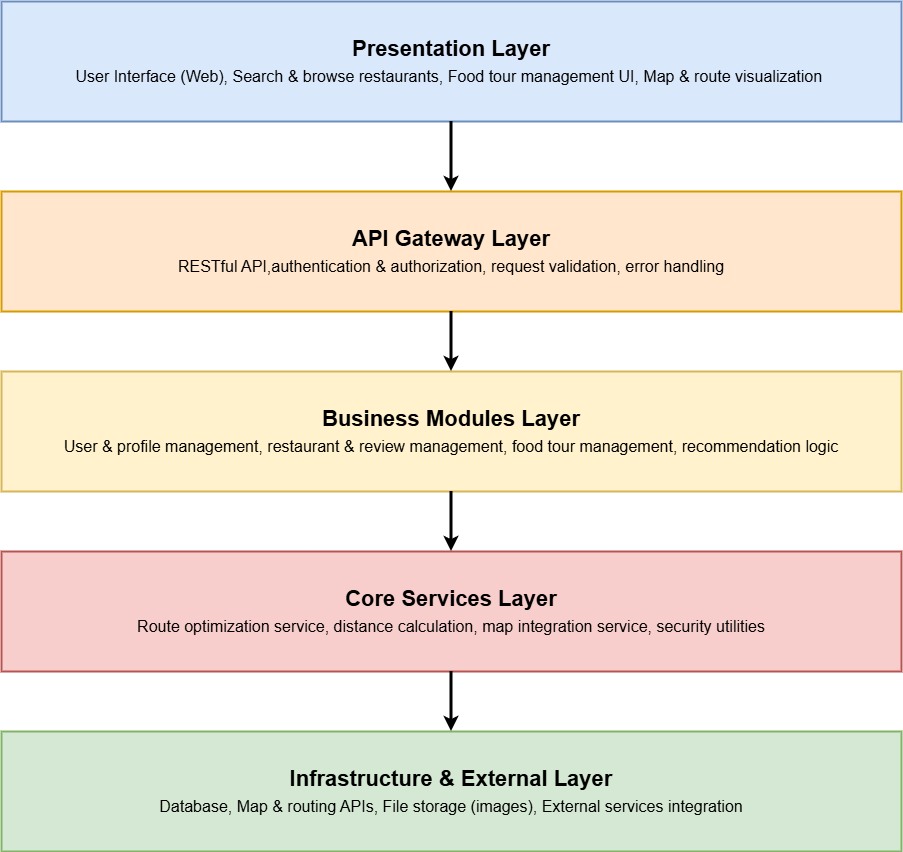
\includegraphics[width=0.85\linewidth]{img/3.png}
    \caption{Layered Architecture}
\end{figure}

Hệ thống được tổ chức theo kiến trúc phân lớp nhằm đảm bảo nguyên tắc tách biệt trách nhiệm (separation of concerns), giúp tăng khả năng mở rộng, bảo trì và kiểm thử hệ thống. Kiến trúc bao gồm 5 lớp chính, được minh họa trong Hình 5.1. Các lớp chính bao gồm:
\begin{itemize}[label=\textbullet]
    \item \textbf{Presentation Layer (Lớp trình bày)}: Lớp trình bày chịu trách nhiệm cung cấp giao diện tương tác trực tiếp với người dùng. Lớp này cho phép người dùng thực hiện các chức năng như tìm kiếm và duyệt quán ăn, tạo và quản lý food tour, xem bản đồ và lộ trình di chuyển, cũng như lưu/yêu thích và chia sẻ food tour.
Presentation Layer tập trung vào trải nghiệm người dùng, điều hướng trang và hiển thị dữ liệu; không xử lý logic nghiệp vụ.
    \item \textbf{API Gateway Layer}: API Gateway Layer đóng vai trò là lớp trung gian giữa Presentation Layer và các lớp xử lý nghiệp vụ bên trong hệ thống. Lớp này chịu trách nhiệm tiếp nhận các yêu cầu từ phía client, thực hiện xác thực và phân quyền truy cập, kiểm tra tính hợp lệ của dữ liệu đầu vào, cũng như xử lý lỗi và chuẩn hóa phản hồi trước khi chuyển yêu cầu xuống các lớp bên dưới.
    \item \textbf{Business Modules Layer}: Business Modules Layer chứa các module nghiệp vụ chính của hệ thống, tương ứng với các ca sử dụng đã được phân tích. Các module tiêu biểu bao gồm:
    \begin{itemize}[label=\textbullet]
        \item Quản lý người dùng và hồ sơ cá nhân.
        \item Quản lý quán ăn và đánh giá.
        \item Quản lý food tour và các điểm dừng.
        \item Xử lý logic gợi ý dựa trên mức độ tương đồng.
    \end{itemize}
    Lớp này chịu trách nhiệm điều phối nghiệp vụ và áp dụng các quy tắc xử lý ở mức ứng dụng.
    \item \textbf{Core Services Layer}: Core Services Layer cung cấp các dịch vụ dùng chung cho toàn hệ thống, bao gồm các chức năng xử lý chuyên sâu như tối ưu lộ trình di chuyển, tính toán khoảng cách giữa các địa điểm, tích hợp và xử lý dữ liệu bản đồ, cũng như các tiện ích liên quan đến bảo mật.
Các dịch vụ tại lớp này được thiết kế độc lập để có thể tái sử dụng cho nhiều module nghiệp vụ khác nhau.
    \item \textbf{Infrastructure \& External Layer}: Lớp hạ tầng và dịch vụ ngoài chịu trách nhiệm quản lý việc lưu trữ và truy xuất dữ liệu, cũng như tích hợp với các hệ thống bên ngoài. Lớp này bao gồm hệ quản trị cơ sở dữ liệu, các API bản đồ và định tuyến, dịch vụ lưu trữ hình ảnh và các dịch vụ ngoài khác.
Việc tách riêng lớp hạ tầng giúp hệ thống giảm sự phụ thuộc vào công nghệ cụ thể và thuận tiện cho việc thay đổi hoặc mở rộng trong tương lai.
\end{itemize}

\textbf{Nhận xét chung}:
Kiến trúc phân lớp giúp hệ thống được tổ chức rõ ràng, dễ kiểm soát, hỗ trợ kiểm thử theo từng mức (unit test, integration test), đồng thời tạo điều kiện thuận lợi cho việc phát triển và mở rộng hệ thống theo hướng module hóa.

\subsubsection{Lý do lựa chọn kiến trúc}
Việc lựa chọn kiến trúc phân lớp cho hệ thống xuất phát từ các yêu cầu của đề tài:
\begin{itemize}[label=\textbullet]
    \item \textbf{Dễ phát triển và mở rộng}: mỗi lớp có thể được mở rộng mà ít ảnh hưởng đến các lớp khác (ví dụ: bổ sung tiêu chí tìm kiếm, thay đổi thuật toán tối ưu lộ trình).
    \item \textbf{Dễ bảo trì}: logic nghiệp vụ tập trung tại các lớp dịch vụ/nghiệp vụ, giảm lặp và dễ kiểm soát.
    \item \textbf{Phù hợp với hệ thống web hướng dịch vụ}: các chức năng có thể được tổ chức thành các dịch vụ rõ ràng tương ứng với các ca sử dụng đã phân tích.
\end{itemize}

% ====================== BỔ SUNG PHẦN GỢI Ý QUÁN ĂN ======================
\subsection{Thiết kế module Gợi ý quán ăn}
Module Gợi ý quán ăn là một trong những module quan trọng của hệ thống, nhằm cung cấp trải nghiệm cá nhân hóa cho người dùng. Module này được thiết kế theo cách hybrid, kết hợp nhiều tiêu chí để đưa ra danh sách gợi ý phù hợp nhất.

Các thành phần chính của module bao gồm:
\begin{itemize}[label=\textbullet]
    \item Phân tích khẩu vị cá nhân (taste profile) và khu vực ưu tiên của người dùng.
    \item Tính toán độ tương đồng giữa khẩu vị người dùng với đặc điểm của các quán ăn (category matching).
    \item Xem xét lịch sử food tour của người dùng để ưu tiên các quán đã từng xuất hiện.
    \item Kết hợp vị trí hiện tại để ưu tiên quán ăn gần nhất.
    \item Hiển thị lý do gợi ý rõ ràng cho từng quán (ví dụ: “Bạn thích món cay • Đã xuất hiện trong 2 food tour trước”).
\end{itemize}

Module này được tích hợp trực tiếp vào giao diện tạo và quản lý food tour, giúp người dùng nhận gợi ý ngay khi đang xây dựng hành trình.

% ====================== KẾT THÚC BỔ SUNG ======================

\subsection{Thiết kế cơ sở dữ liệu}
\subsubsection{ERD}
ERD tổng quan của toàn bộ hệ thống được biểu diễn ở hình 5.2
\begin{figure}[H]
    \centering
    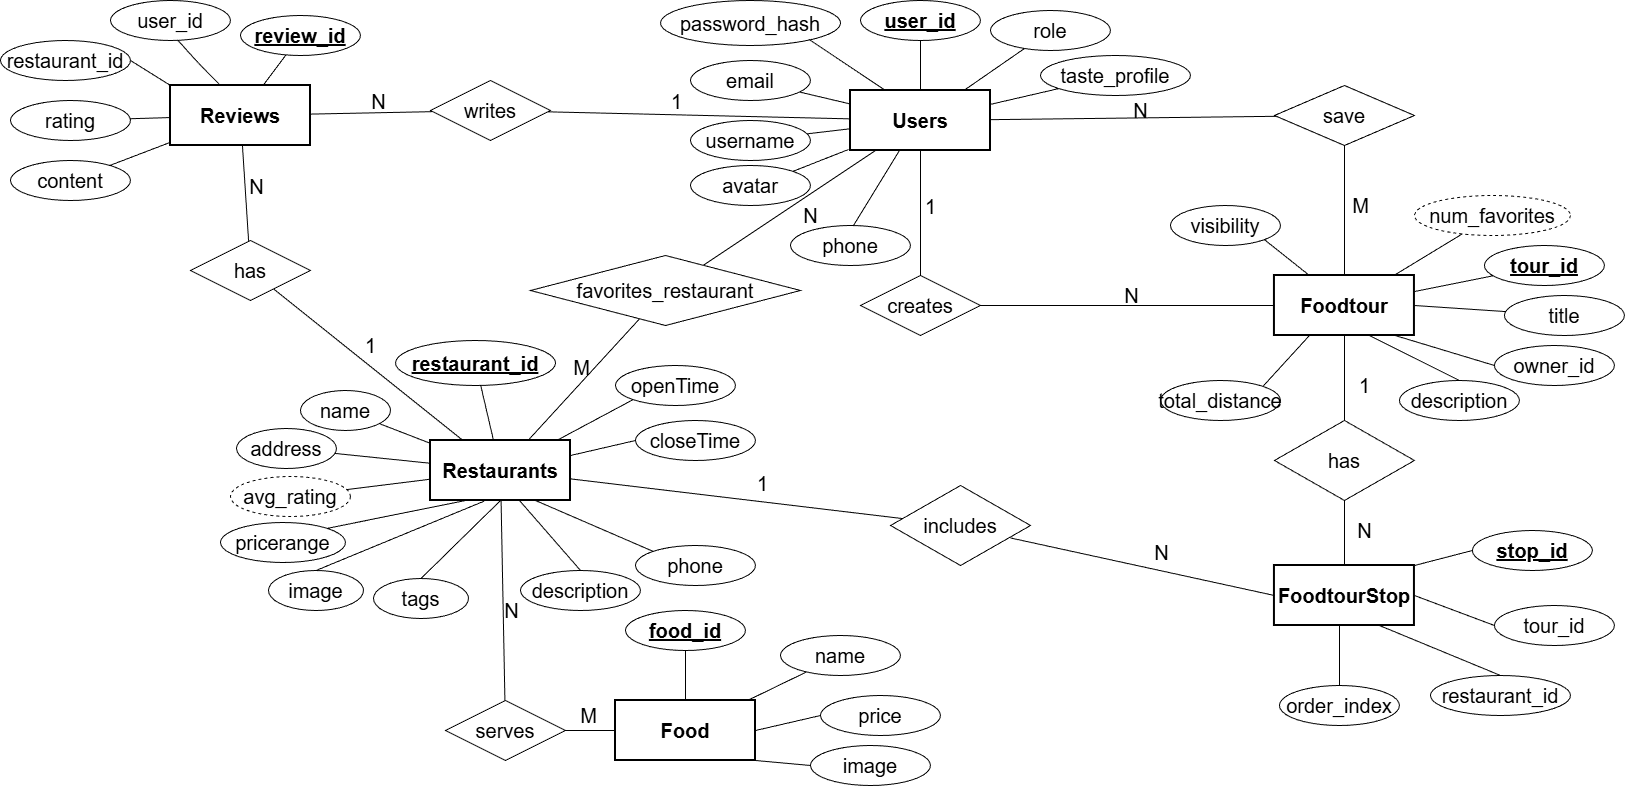
\includegraphics[page=1, angle=-90,width=0.63\textwidth]{img/2.png}
    \caption{Lược đồ ERD}
\end{figure}

\subsubsubsection{Thực thể Users}
\begin{itemize}[label=\textbullet]
    \item \textbf{Thuộc tính}:
    \begin{itemize}
        \item user\_id (khóa chính)
        \item email
        \item username
        \item password\_hash
        \item phone
        \item avatar
        \item role
        \item taste\_profile
    \end{itemize}
    \item \textbf{Quan hệ}:
    \begin{itemize}
        \item Writes – với Reviews (1--N)
        \item Creates – với Foodtour (1--N)
        \item Save – với Foodtour (N--M)
        \item Favorites\_restaurant – với Restaurants (N--M)
    \end{itemize}
\end{itemize}

\subsubsubsection{Thực thể Restaurants}
\begin{itemize}[label=\textbullet]
    \item \textbf{Thuộc tính}:
    \begin{itemize}
        \item restaurant\_id (khóa chính)
        \item name
        \item address
        \item phone
        \item description
        \item image
        \item tags
        \item priceRange
        \item openTime
        \item closeTime
        \item avg\_rating (thuộc tính dẫn xuất)
    \end{itemize}
    \item \textbf{Quan hệ}:
    \begin{itemize}
        \item Has – với Reviews (1--N)
        \item Includes – với FoodtourStop (1--N)
        \item Serves – với Food (N--M)
        \item Favorites\_restaurant – với Users (N--M)
    \end{itemize}
\end{itemize}

\subsubsubsection{Thực thể Reviews}
\begin{itemize}[label=\textbullet]
    \item \textbf{Thuộc tính}:
    \begin{itemize}
        \item review\_id (khóa chính)
        \item user\_id
        \item restaurant\_id
        \item rating
        \item content
    \end{itemize}
    \item \textbf{Quan hệ}:
    \begin{itemize}
        \item Writes – với Users (N--1)
        \item Has – với Restaurants (N--1)
    \end{itemize}
\end{itemize}

\subsubsubsection{Thực thể Foodtour}
\begin{itemize}[label=\textbullet]
    \item \textbf{Thuộc tính}:
    \begin{itemize}
        \item tour\_id (khóa chính)
        \item title
        \item description
        \item visibility
        \item owner\_id
        \item total\_distance
        \item num\_favorites (thuộc tính dẫn xuất)
    \end{itemize}
    \item \textbf{Quan hệ}:
    \begin{itemize}
        \item Creates – với Users (N--1)
        \item Save – với Users (N--M)
        \item Has – với FoodtourStop (1--N)
    \end{itemize}
\end{itemize}

\subsubsubsection{Thực thể FoodtourStop}
\begin{itemize}[label=\textbullet]
    \item \textbf{Thuộc tính}:
    \begin{itemize}
        \item stop\_id (khóa chính)
        \item tour\_id
        \item restaurant\_id
        \item order\_index
    \end{itemize}
    \item \textbf{Quan hệ}:
    \begin{itemize}
        \item Has – với Foodtour (N--1)
        \item Includes – với Restaurants (N--1)
    \end{itemize}
\end{itemize}

\subsubsubsection{Thực thể Food}
\begin{itemize}[label=\textbullet]
    \item \textbf{Thuộc tính}:
    \begin{itemize}
        \item food\_id (khóa chính)
        \item name
        \item price
        \item image
    \end{itemize}
    \item \textbf{Quan hệ}:
    \begin{itemize}
        \item Serves – với Restaurants (N--M)
    \end{itemize}
\end{itemize}


\subsubsection{Collection Schema}
Sau khi xây dựng mô hình dữ liệu ở mức logic thông qua ERD, hệ thống được thiết kế cơ sở dữ liệu theo mô hình hướng document phù hợp với MongoDB. Phần này trình bày schema của các collection chính trong hệ thống, cách tổ chức dữ liệu và cơ chế liên kết giữa các collection nhằm đáp ứng yêu cầu nghiệp vụ và tối ưu hiệu năng truy vấn.
\begin{figure}[H]
    \centering
    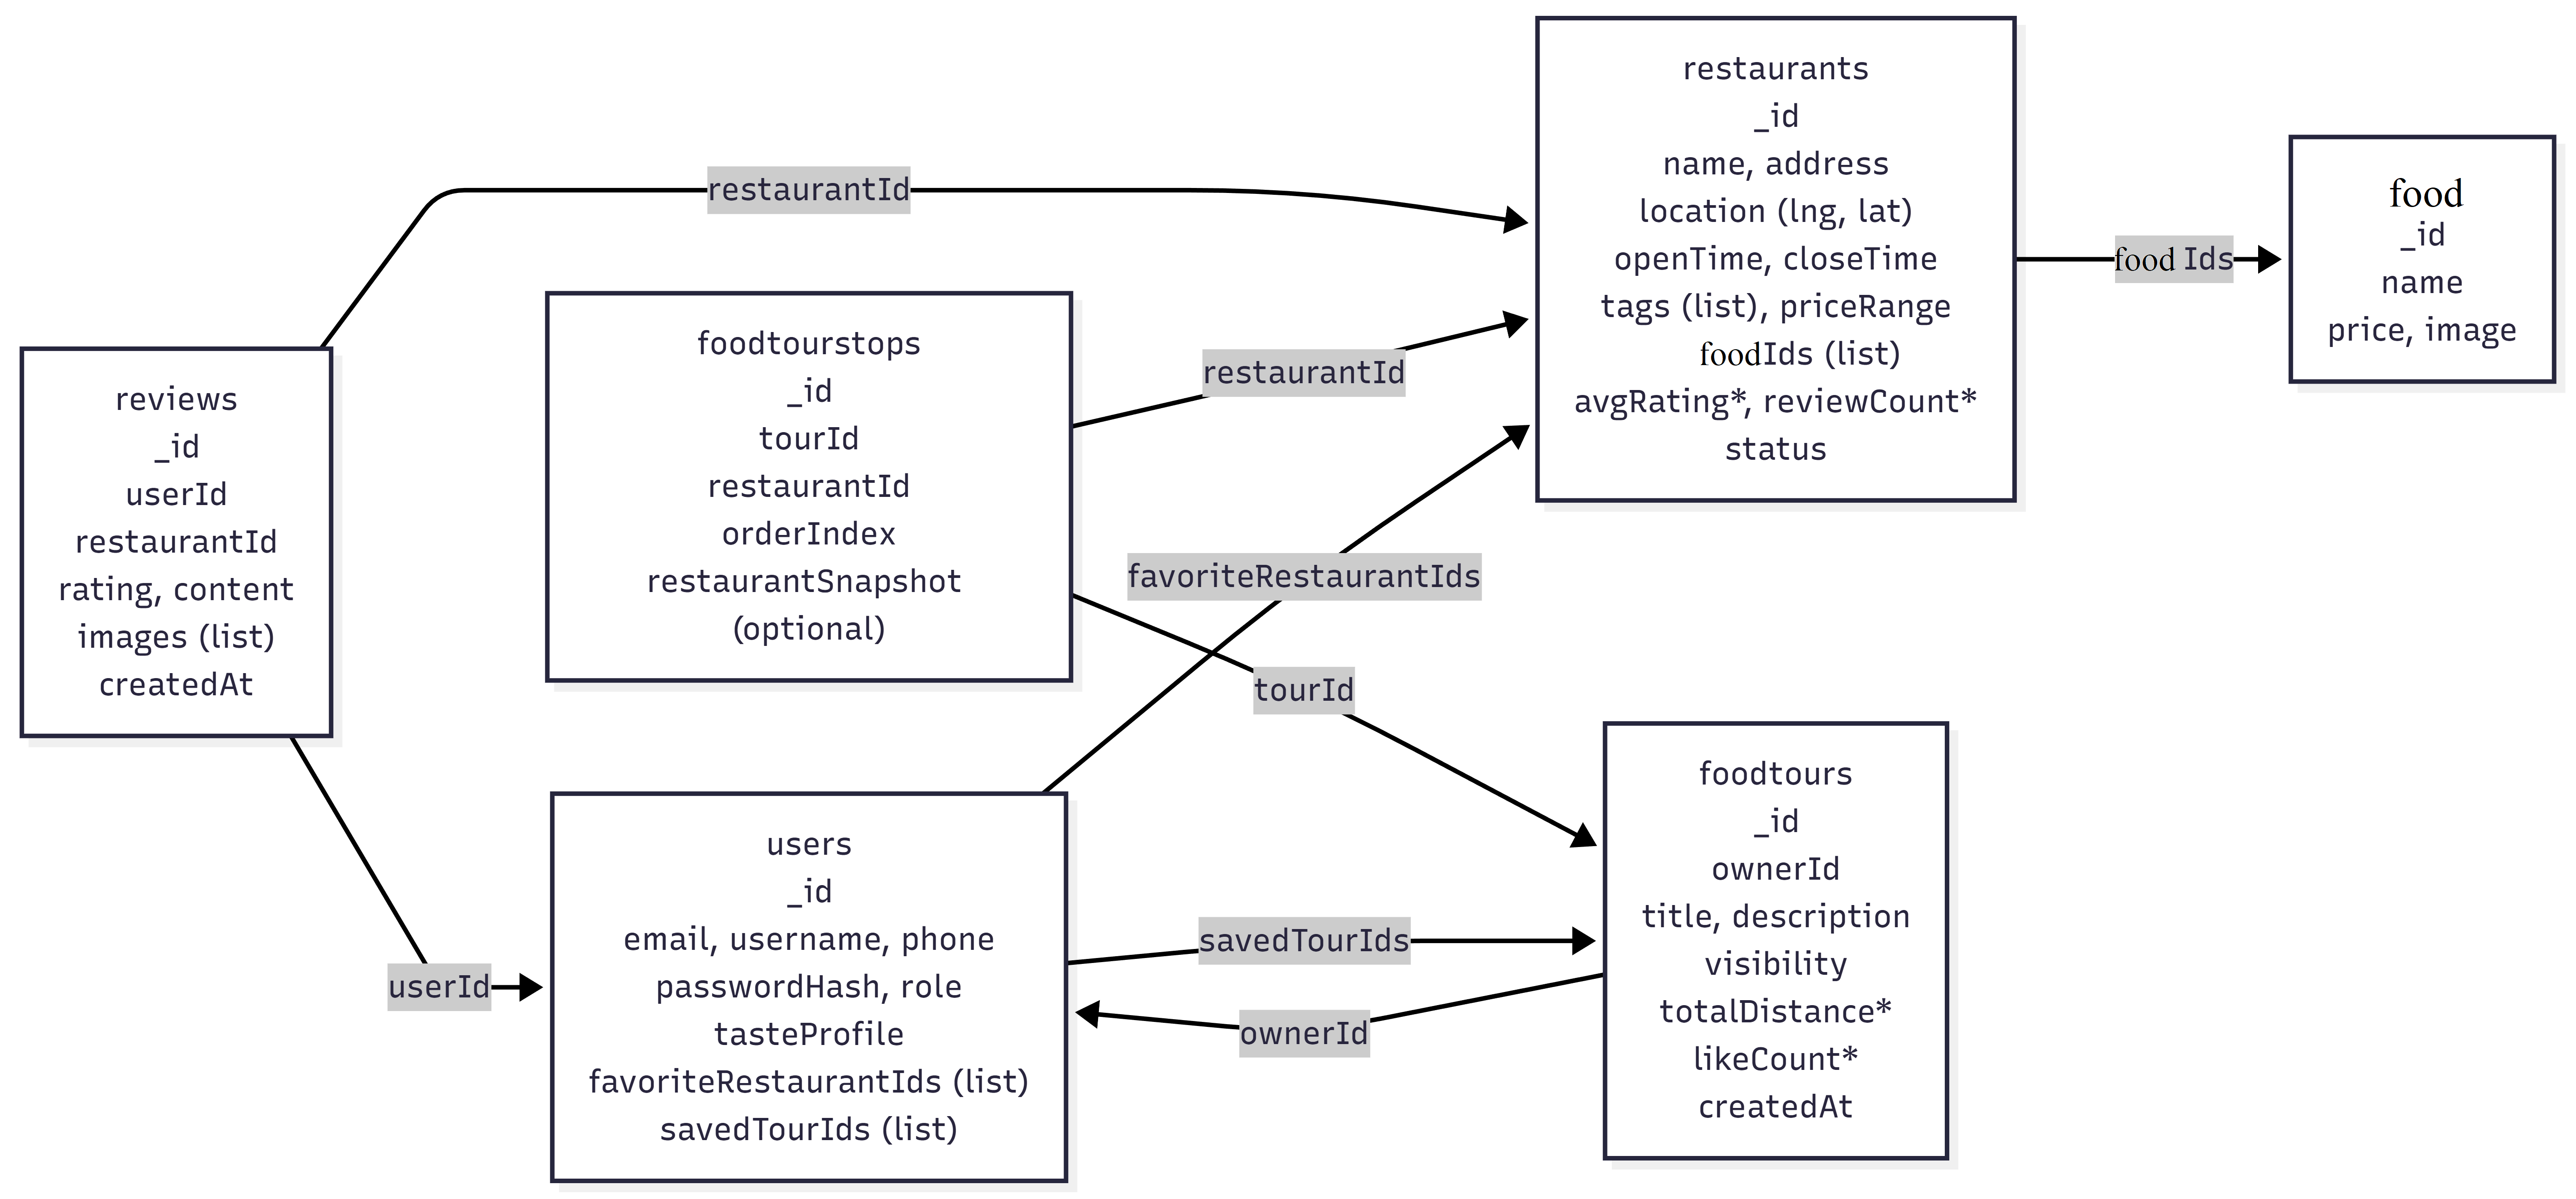
\includegraphics[page=1, angle=-90,width=0.68\textwidth]{img/5.png}
    \caption{Collection Schema Diagram}
\end{figure}

Hình 5.3 minh họa lược đồ dữ liệu mức logic của hệ thống CityFoodTour, được thiết kế theo mô hình hướng tài liệu (document-oriented) của cơ sở dữ liệu MongoDB. Lược đồ thể hiện các collection chính của hệ thống cùng mối quan hệ logic giữa chúng thông qua các trường tham chiếu (reference), phù hợp với đặc thù schema linh hoạt của NoSQL.

Collection users lưu trữ thông tin người dùng, bao gồm các thuộc tính cơ bản như email, tên người dùng, số điện thoại, mật khẩu đã mã hóa và vai trò trong hệ thống. Ngoài ra, collection này còn lưu trữ hồ sơ khẩu vị (tasteProfile), danh sách các quán ăn yêu thích (favoriteRestaurantIds) và các food tour đã lưu (savedTourIds), phục vụ cho việc cá nhân hóa trải nghiệm người dùng.

Collection restaurants quản lý thông tin các quán ăn trong hệ thống, bao gồm tên quán, địa chỉ, vị trí địa lý (kinh độ, vĩ độ), thời gian mở cửa – đóng cửa, các thẻ phân loại, mức giá và danh sách loại hình ẩm thực (foodIds). Các thông tin tổng hợp như điểm đánh giá trung bình và số lượng đánh giá được lưu trữ nhằm tối ưu hiệu năng truy vấn.

Collection reviews lưu trữ các đánh giá của người dùng đối với quán ăn. Mỗi đánh giá liên kết với một người dùng (userId) và một quán ăn (restaurantId), bao gồm nội dung nhận xét, điểm đánh giá, hình ảnh kèm theo và thời điểm tạo đánh giá. Collection này đóng vai trò cung cấp dữ liệu phản hồi cho cộng đồng người dùng.

Collection foodtours đại diện cho các hành trình ăn uống do người dùng tạo. Mỗi food tour liên kết với người tạo thông qua trường ownerId, đồng thời lưu trữ các thông tin mô tả như tiêu đề, mô tả, trạng thái hiển thị (công khai hoặc riêng tư), tổng quãng đường di chuyển và số lượt yêu thích. Các trường tổng hợp được tính toán và lưu sẵn nhằm hỗ trợ hiển thị nhanh trên giao diện.

Collection foodtourstops đóng vai trò trung gian, mô tả các điểm dừng trong một food tour. Mỗi bản ghi liên kết đến một food tour (tourId) và một quán ăn (restaurantId), kèm theo thứ tự ghé thăm (orderIndex). Ngoài ra, hệ thống cho phép lưu trữ thông tin snapshot của quán ăn tại thời điểm tạo food tour nhằm đảm bảo tính nhất quán dữ liệu khi thông tin quán ăn thay đổi.

Bên cạnh đó, collection food được sử dụng để quản lý các món ăn, bao gồm tên món, giá và hình ảnh, đồng thời liên kết với quán ăn thông qua danh sách loại hình ẩm thực. Việc sử dụng các trường tham chiếu thay cho quan hệ ràng buộc cứng giúp hệ thống linh hoạt, dễ mở rộng và phù hợp với kiến trúc NoSQL.

\subsection{Thiết kế giao diện}
\subsubsection{Nguyên tắc thiết kế}
Thiết kế giao diện người dùng (User Interface – UI) đóng vai trò quan trọng trong việc nâng cao trải nghiệm sử dụng và hiệu quả tương tác giữa người dùng và hệ thống. Đối với hệ thống FoodTour Planner, giao diện được thiết kế dựa trên các nguyên tắc cơ bản nhằm đảm bảo tính dễ sử dụng, trực quan và phù hợp với nhiều nhóm người dùng khác nhau. Các nguyên tắc thiết kế chính được áp dụng bao gồm:
\subsubsubsection{Tính nhất quán}
Giao diện hệ thống cần đảm bảo tính nhất quán trong cách bố trí, màu sắc, kiểu chữ và cách thức tương tác trên toàn bộ các trang. Các thành phần giao diện như thanh điều hướng, nút chức năng, biểu tượng và thông báo được sử dụng đồng nhất nhằm giúp người dùng dễ dàng ghi nhớ và làm quen với hệ thống. Tính nhất quán giúp giảm thời gian học cách sử dụng, hạn chế nhầm lẫn và tăng hiệu quả thao tác.
\subsubsubsection{Tính đơn giản}
Giao diện được thiết kế theo hướng đơn giản, tập trung vào các chức năng cốt lõi và hạn chế các thành phần không cần thiết. Thông tin được trình bày ngắn gọn, rõ ràng, tránh gây quá tải cho người dùng. Việc đơn giản hóa giao diện giúp người dùng nhanh chóng thực hiện các thao tác chính như tìm kiếm quán ăn, tạo food tour và xem lộ trình di chuyển mà không cần nhiều bước phức tạp.
\subsubsubsection{Khả năng tiếp cận}
Hệ thống được thiết kế để có thể tiếp cận dễ dàng đối với nhiều đối tượng người dùng khác nhau, bao gồm cả những người không có nhiều kiến thức kỹ thuật. Giao diện sử dụng màu sắc có độ tương phản phù hợp, kích thước chữ dễ đọc và bố cục rõ ràng. Các thành phần tương tác được thiết kế đủ lớn và dễ thao tác trên cả thiết bị máy tính và thiết bị di động, nhằm nâng cao khả năng sử dụng trong nhiều ngữ cảnh khác nhau.
\subsubsubsection{Phản hồi trực quan}
Mọi thao tác của người dùng trên hệ thống đều cần có phản hồi trực quan để giúp người dùng nhận biết trạng thái hiện tại của hệ thống. Các hành động như đăng nhập, thêm quán ăn vào food tour, tối ưu lộ trình hay lưu food tour đều được hiển thị thông báo thành công hoặc thất bại tương ứng. Ngoài ra, các hiệu ứng trực quan như thay đổi màu sắc nút bấm hoặc hiển thị trạng thái tải dữ liệu giúp tăng tính tương tác và giảm cảm giác chờ đợi cho người dùng.
\subsubsubsection{Phân cấp thông tin}
Thông tin trên giao diện được tổ chức theo mức độ quan trọng, giúp người dùng dễ dàng tập trung vào các nội dung chính. Các thông tin quan trọng như tên food tour, danh sách quán ăn, tổng khoảng cách di chuyển và bản đồ lộ trình được ưu tiên hiển thị nổi bật. Các thông tin bổ trợ được sắp xếp hợp lý ở các khu vực phụ, tránh làm rối bố cục tổng thể. Việc phân cấp thông tin hợp lý giúp người dùng nhanh chóng nắm bắt nội dung và đưa ra quyết định hiệu quả.
\subsubsection{Thiết kế luồng giao diện hệ thống}
Luồng giao diện hệ thống (User Interface Workflow) được xây dựng nhằm mô tả cách
người dùng và quản trị viên tương tác với hệ thống thông qua các màn hình giao diện
chính. Thông qua sơ đồ luồng giao diện, có thể hình dung tổng thể quá trình điều hướng
giữa các trang, từ khi người dùng truy cập hệ thống cho đến khi thực hiện các chức năng
chính như tìm kiếm quán ăn, quản lý food tour hoặc quản trị dữ liệu hệ thống.

Trong sơ đồ luồng giao diện, mỗi hình chữ nhật đại diện cho một màn hình giao diện
của hệ thống, trong khi các mũi tên biểu diễn luồng điều hướng giữa các màn hình thông
qua thao tác của người dùng hoặc quản trị viên. User interface workflow của hệ thống được biểu diễn ở Hình 5.4
\begin{figure}[H]
    \centering
    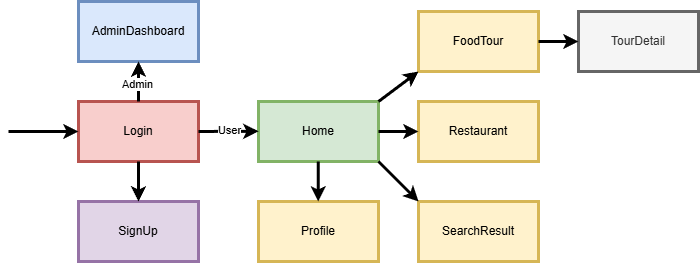
\includegraphics[width=1\textwidth]{img/workflow.png}
    \caption{User Interface Workflow}
\end{figure}

\subsubsection{Chi tiết giao diện hệ thống}
\subsubsubsection{Giao diện đăng nhập}
Hình 5.5 minh họa giao diện đăng nhập của hệ thống CityFoodTour. Đây là màn hình
đầu tiên mà người dùng tương tác khi truy cập vào hệ thống, cho phép người dùng
xác thực tài khoản để sử dụng các chức năng chính.

\begin{figure}[H]
    \centering
    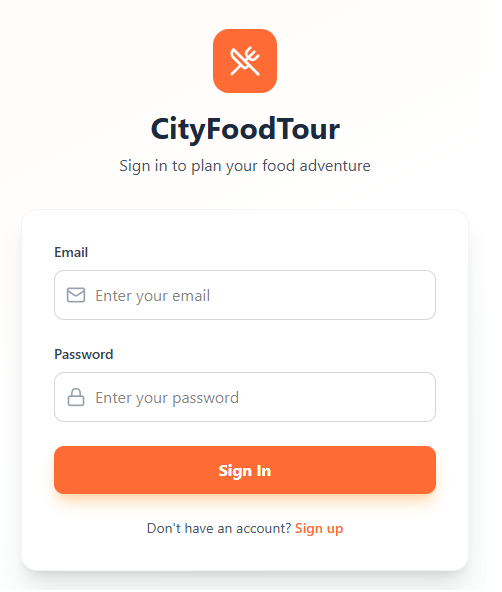
\includegraphics[width=0.8\textwidth]{img/signup.png}
    \caption{Giao diện đăng nhập}
\end{figure}

Giao diện đăng nhập yêu cầu người dùng nhập thông tin email và mật khẩu đã được
đăng ký trước đó. Các trường nhập liệu được thiết kế rõ ràng, có nhãn mô tả cụ thể nhằm giúp người dùng dễ dàng nhận biết và thao tác. Nút đăng nhập được đặt ở vị trí trung tâm, nổi bật, hỗ trợ người dùng nhanh chóng hoàn tất quá trình đăng nhập.

Ngoài ra, giao diện cung cấp liên kết chuyển sang chức năng đăng ký tài khoản mới (Sign up) dành cho người dùng chưa có tài khoản. Việc bố trí liên kết này ngay trên màn hình đăng nhập giúp tăng tính thuận tiện và đảm bảo luồng sử dụng liên tục trong quá trình tương tác với hệ thống.

Về mặt thiết kế, giao diện được xây dựng theo hướng đơn giản và nhất quán với tổng thể hệ thống, tập trung vào chức năng cốt lõi và hạn chế các thành phần không cần thiết. Hệ thống đồng thời cung cấp phản hồi trực quan khi thông tin đăng nhập không hợp lệ, giúp người dùng dễ dàng nhận biết và điều chỉnh thao tác.
\subsubsubsection{Giao diện quản trị hệ thống}
Hình 5.6 minh họa giao diện quản trị hệ thống (Admin Dashboard), được thiết kế dành riêng cho quản trị viên nhằm hỗ trợ việc giám sát và quản lý dữ liệu của hệ thống CityFoodTour.

\begin{figure}[H]
    \centering
    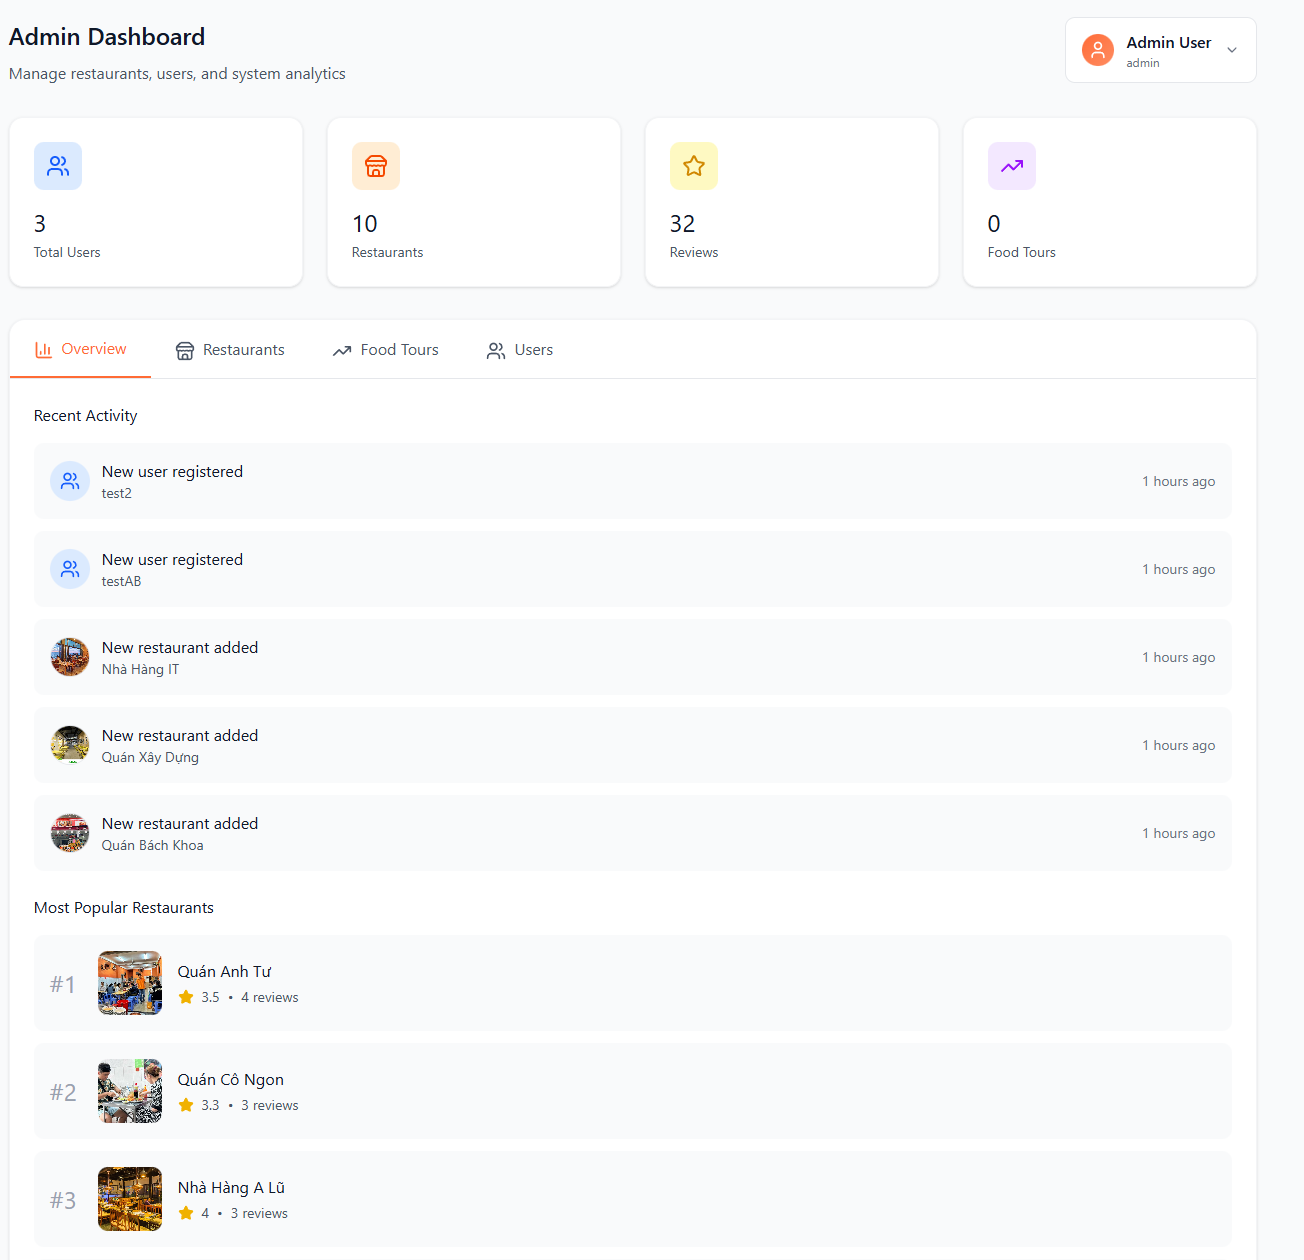
\includegraphics[width=1\textwidth]{img/admin.png}
    \caption{Giao diện quản trị hệ thống}
\end{figure}
Giao diện dashboard cung cấp các thông tin thống kê tổng quan, bao gồm tổng số
người dùng, số lượng quán ăn, số lượt đánh giá và số lượng food tour hiện có trong hệ thống. Các chỉ số này được hiển thị trực quan, giúp quản trị viên nhanh chóng nắm bắt tình trạng hoạt động chung của hệ thống.

Trong mục Overview, hệ thống hiển thị các hoạt động gần đây liên quan đến người
dùng, quán ăn và food tour, chẳng hạn như đăng ký người dùng mới hoặc cập nhật dữ liệu quán ăn. Bên cạnh đó, giao diện cũng cung cấp danh sách các quán ăn phổ biến dựa trên số lượt đánh giá, hỗ trợ quản trị viên theo dõi mức độ tương tác của người dùng.

Giao diện quản trị cho phép quản trị viên thực hiện các chức năng quản lý dữ liệu nền tảng thông qua các mục chức năng riêng biệt. Trong mục Restaurants, quản trị viên có thể thêm, chỉnh sửa hoặc xóa thông tin quán ăn. Trong mục Users, quản trị viên có thể quản lý tài khoản người dùng, bao gồm các thao tác xóa tài khoản, khóa hoặc mở khóa người dùng khi cần thiết. Trong mục food tour, quản trị viên có thể duyệt hoặc xóa food tour ở chế độ public của người dùng.

Nhìn chung, giao diện Admin Dashboard được thiết kế đơn giản, rõ ràng và nhất quán với tổng thể hệ thống, tập trung vào các chức năng quản lý cốt lõi nhằm đảm bảo hệ thống hoạt động ổn định và hiệu quả.

\subsubsubsection{Giao diện trang chủ}
Giao diện trang chủ (Home) là màn hình trung tâm của hệ thống CityFoodTour, đóng
vai trò là điểm khởi đầu cho hầu hết các thao tác của người dùng sau khi đăng nhập. Giao diện này được thiết kế nhằm cung cấp cái nhìn tổng quan về hệ thống cũng như hỗ trợ người dùng nhanh chóng tiếp cận các chức năng chính.

Hình 5.7 minh họa giao diện trang chủ của hệ thống. Tại khu vực đầu trang, hệ thống hiển thị thanh tìm kiếm và bộ lọc cho phép người dùng tra cứu quán ăn theo nhiều tiêu chí khác nhau như loại ẩm thực, vị trí, thời gian mở cửa, mức đánh giá và ngân sách. Việc tích hợp các bộ lọc này ngay trên trang chủ giúp người dùng dễ dàng bắt đầu quá trình tìm kiếm mà không cần chuyển sang màn hình khác.

\begin{figure}[H]
    \centering
    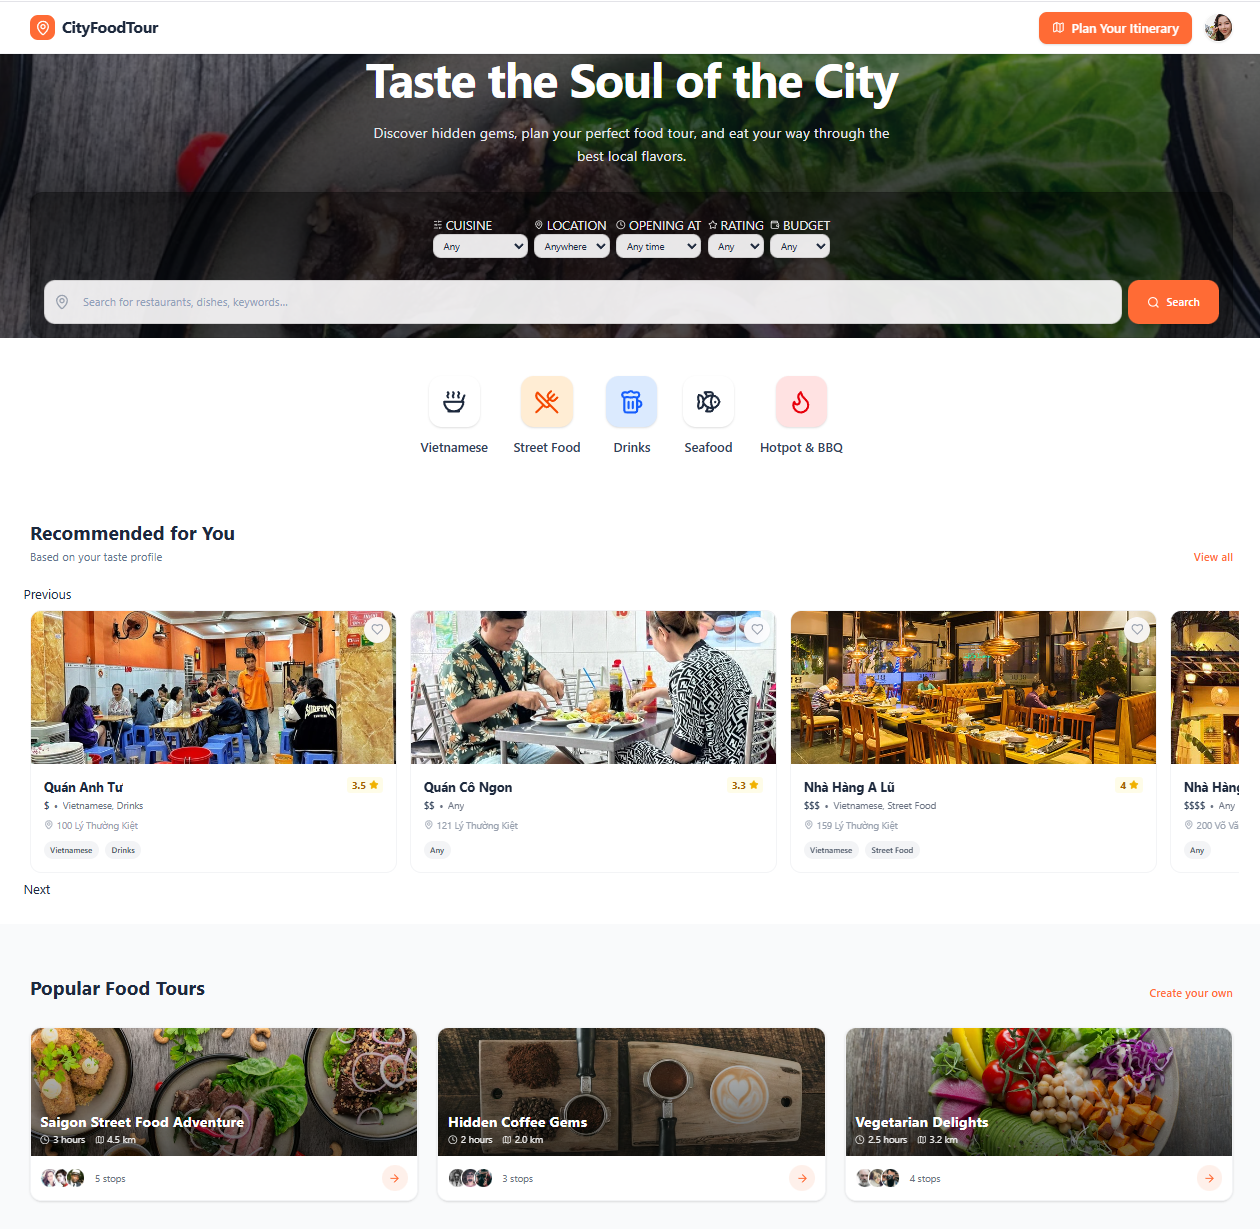
\includegraphics[width=1\textwidth]{img/home.png}
    \caption{Giao diện trang chủ}
\end{figure}
Bên dưới khu vực tìm kiếm, giao diện cung cấp các danh mục ẩm thực phổ biến dưới
dạng biểu tượng, hỗ trợ người dùng khám phá nhanh các nhóm quán ăn theo sở thích. Ngoài ra, hệ thống hiển thị danh sách các quán ăn được đề xuất dựa trên hồ sơ khẩu vị của người dùng, giúp cá nhân hóa trải nghiệm sử dụng.

Trang chủ cũng hiển thị danh sách các food tour phổ biến, cho phép người dùng tham khảo các hành trình ăn uống đã được xây dựng sẵn. Từ đây, người dùng có thể xem chi tiết từng food tour hoặc khởi tạo food tour mới thông qua chức năng lập kế hoạch hành trình.

Nhìn chung, giao diện trang chủ được thiết kế trực quan, rõ ràng và nhất quán với tổng thể hệ thống, đóng vai trò quan trọng trong việc hỗ trợ người dùng khám phá ẩm thực và xây dựng các hành trình ăn uống một cách thuận tiện và hiệu quả.

\subsubsubsection{Giao diện kết quả tìm kiếm}
Giao diện kết quả tìm kiếm được thiết kế nhằm hiển thị danh sách các quán ăn phù hợp với tiêu chí tìm kiếm mà người dùng đã lựa chọn. Đây là giao diện đóng vai trò quan trọng trong việc hỗ trợ người dùng so sánh và lựa chọn quán ăn phù hợp với nhu cầu cá nhân.

Hình 5.8 minh họa giao diện kết quả tìm kiếm của hệ thống. Tại khu vực đầu trang, hệ thống cung cấp thanh tìm kiếm kết hợp với các bộ lọc cho phép người dùng điều chỉnh và tinh chỉnh lại tiêu chí tìm kiếm như loại ẩm thực, vị trí, thời gian mở cửa, mức đánh giá và ngân sách. Việc cho phép thay đổi bộ lọc trực tiếp trên trang kết quả giúp người dùng nhanh chóng cập nhật danh sách quán ăn mà không cần quay lại trang chủ.

\begin{figure}[H]
    \centering
    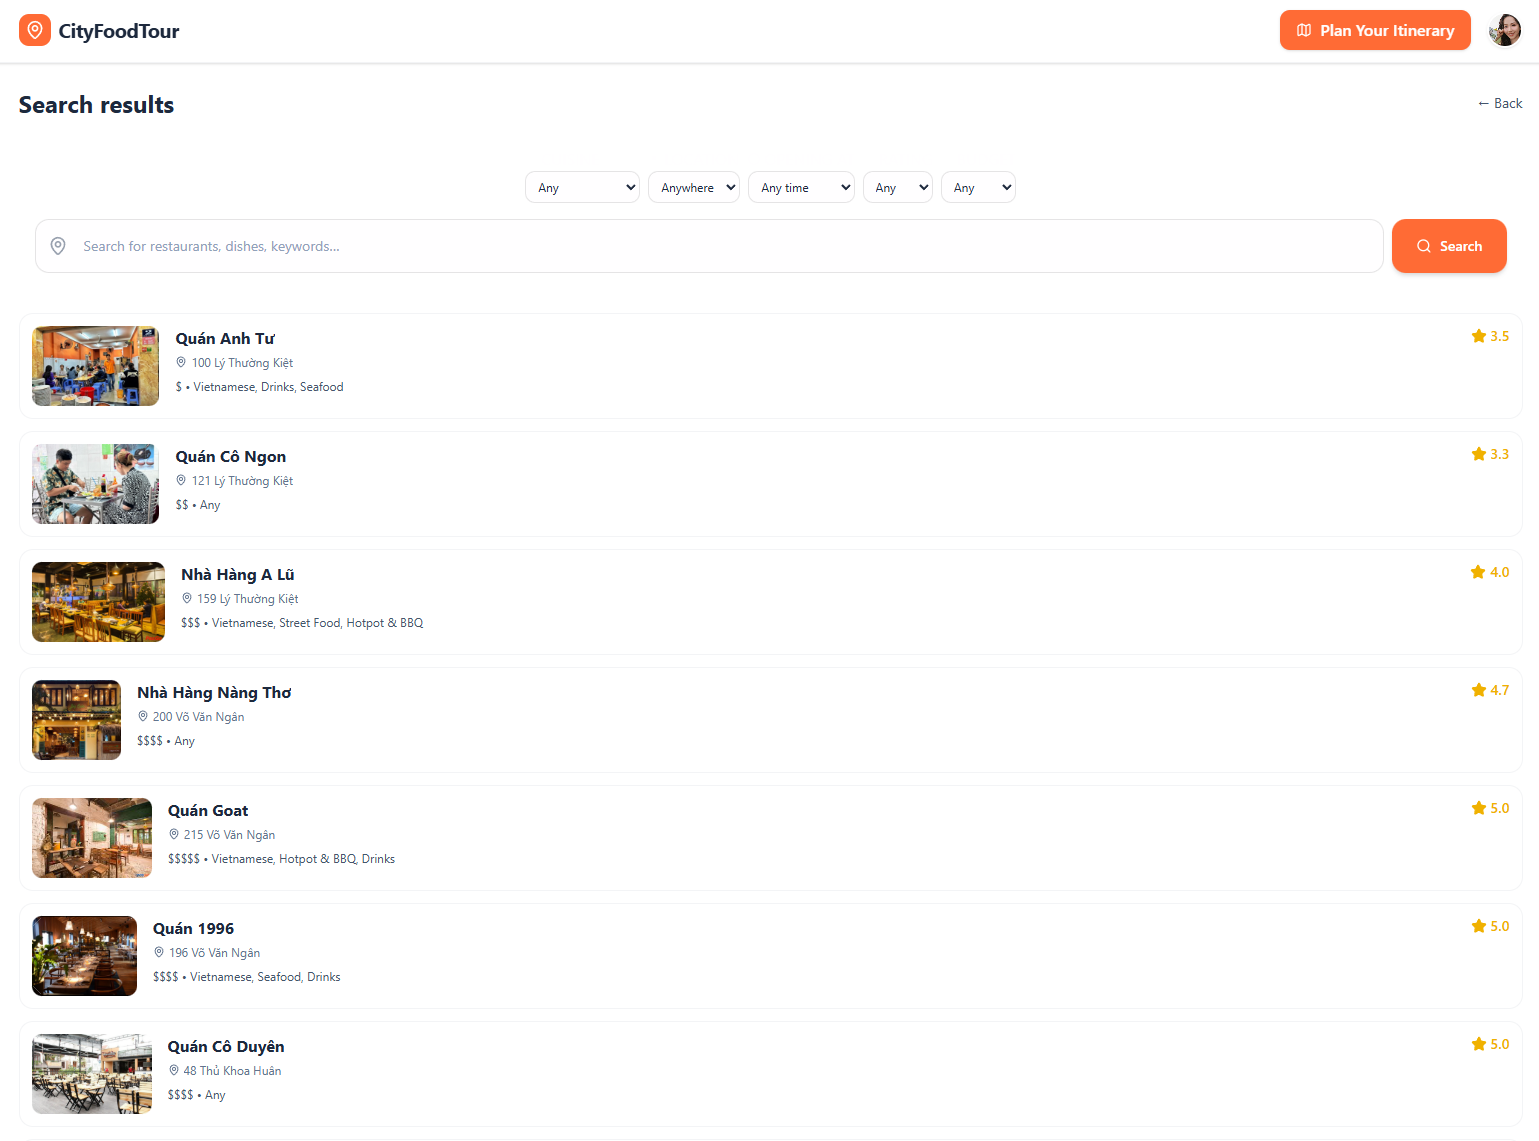
\includegraphics[width=1\textwidth]{img/search.png}
    \caption{Giao diện kết quả tìm kiếm}
\end{figure}

Danh sách kết quả được hiển thị dưới dạng các thẻ thông tin, mỗi thẻ đại diện cho một quán ăn. Thông tin tổng quan của quán ăn bao gồm hình ảnh minh họa, tên quán, địa chỉ, mức giá, loại ẩm thực và điểm đánh giá trung bình. Cách trình bày này giúp người dùng dễ dàng so sánh các lựa chọn và đưa ra quyết định phù hợp.

Ngoài ra, giao diện kết quả tìm kiếm được thiết kế theo hướng đơn giản và dễ theo dõi, đảm bảo các thông tin quan trọng được hiển thị rõ ràng. Người dùng có thể chọn một quán ăn bất kỳ trong danh sách để xem thông tin chi tiết hoặc tiếp tục điều chỉnh tiêu chí tìm kiếm để thu hẹp kết quả.

Nhìn chung, giao diện kết quả tìm kiếm đáp ứng tốt yêu cầu về khả năng sử dụng và hiệu quả tìm kiếm, đóng vai trò cầu nối giữa quá trình tra cứu thông tin và việc lựa chọn quán ăn trong hệ thống CityFoodTour.

\subsubsubsection{Giao diện chi tiết quán ăn}
Giao diện chi tiết quán ăn được thiết kế nhằm cung cấp đầy đủ thông tin về một quán ăn cụ thể, hỗ trợ người dùng đánh giá và quyết định lựa chọn quán ăn phù hợp trong quá trình xây dựng food tour.

Hình 5.9 minh họa giao diện chi tiết quán ăn của hệ thống CityFoodTour. Tại khu vực đầu trang, giao diện hiển thị hình ảnh minh họa, tên quán, điểm đánh giá trung bình và các thông tin tổng quan như loại ẩm thực và trạng thái hoạt động của quán. Các chức năng như xem vị trí trên bản đồ và viết đánh giá được cung cấp nhằm hỗ trợ tương tác trực tiếp với quán ăn.

\begin{figure}[H]
    \centering
    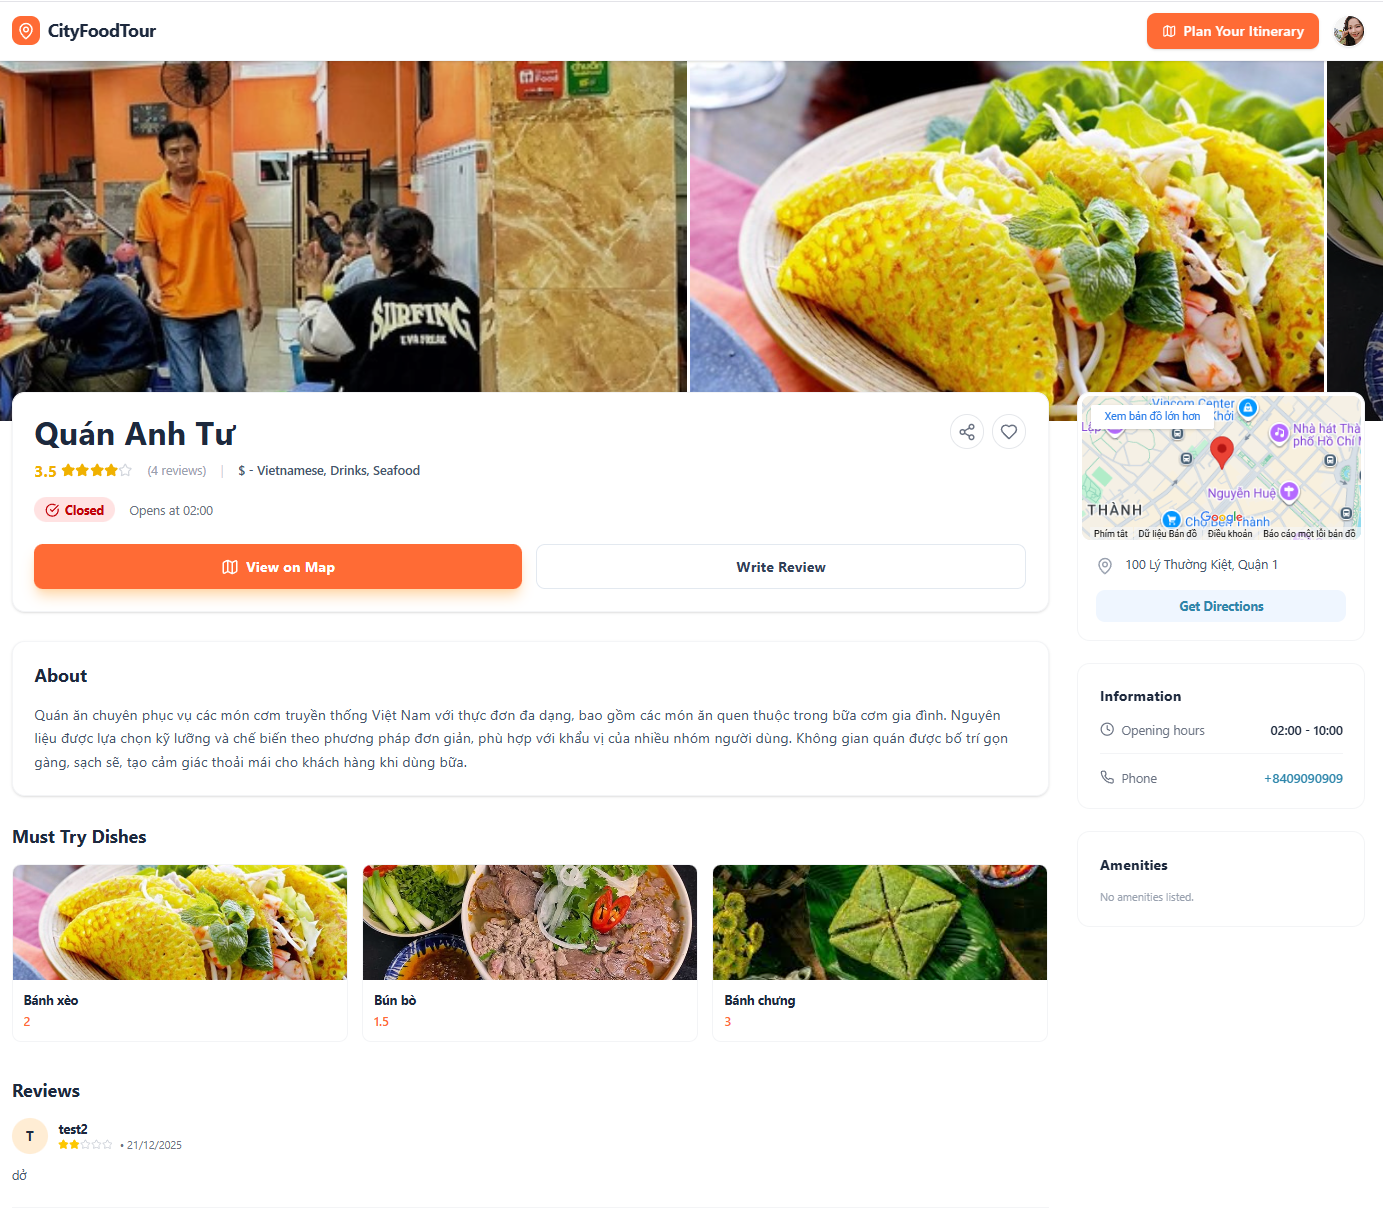
\includegraphics[width=1\textwidth]{img/restaurant.png}
    \caption{Giao diện chi tiết quán ăn}
\end{figure}

Bên cạnh các thông tin tổng quan, giao diện hiển thị bản đồ thu nhỏ giúp người dùng xác định vị trí địa lý của quán ăn và thuận tiện cho việc dẫn đường. Các thông tin liên hệ cơ bản như giờ mở cửa và số điện thoại cũng được hiển thị rõ ràng để phục vụ nhu cầu tham khảo.

Giao diện chi tiết quán ăn còn cung cấp phần mô tả chung về quán, giúp người dùng hiểu rõ hơn về phong cách ẩm thực và không gian phục vụ. Ngoài ra, danh sách các món ăn tiêu biểu được hiển thị kèm hình ảnh minh họa nhằm hỗ trợ người dùng tham khảo trước khi lựa chọn.

Phần đánh giá (Reviews) cho phép người dùng xem các nhận xét và điểm đánh giá từ
những người dùng khác trong hệ thống. Các đánh giá này đóng vai trò quan trọng
trong việc hỗ trợ người dùng đưa ra quyết định lựa chọn quán ăn phù hợp.

Nhìn chung, giao diện chi tiết quán ăn được thiết kế trực quan, đầy đủ thông tin và nhất quán với tổng thể hệ thống, góp phần nâng cao trải nghiệm người dùng trong việc khám phá và lựa chọn địa điểm ăn uống.

\subsubsubsection{Giao diện hồ sơ người dùng}
Giao diện hồ sơ người dùng (Profile) được thiết kế nhằm cho phép người dùng quản
lý thông tin cá nhân và thiết lập các tùy chọn liên quan đến trải nghiệm sử dụng hệ thống CityFoodTour. Đây là giao diện hỗ trợ cá nhân hóa hệ thống dựa trên nhu cầu và sở thích của từng người dùng.

Hình 5.10 minh họa giao diện hồ sơ người dùng của hệ thống. Tại khu vực thông tin cá nhân, giao diện hiển thị các thông tin cơ bản của người dùng như tên hiển thị và thông tin liên hệ, đồng thời cung cấp chức năng chỉnh sửa hồ sơ khi cần thiết.

\begin{figure}[H]
    \centering
    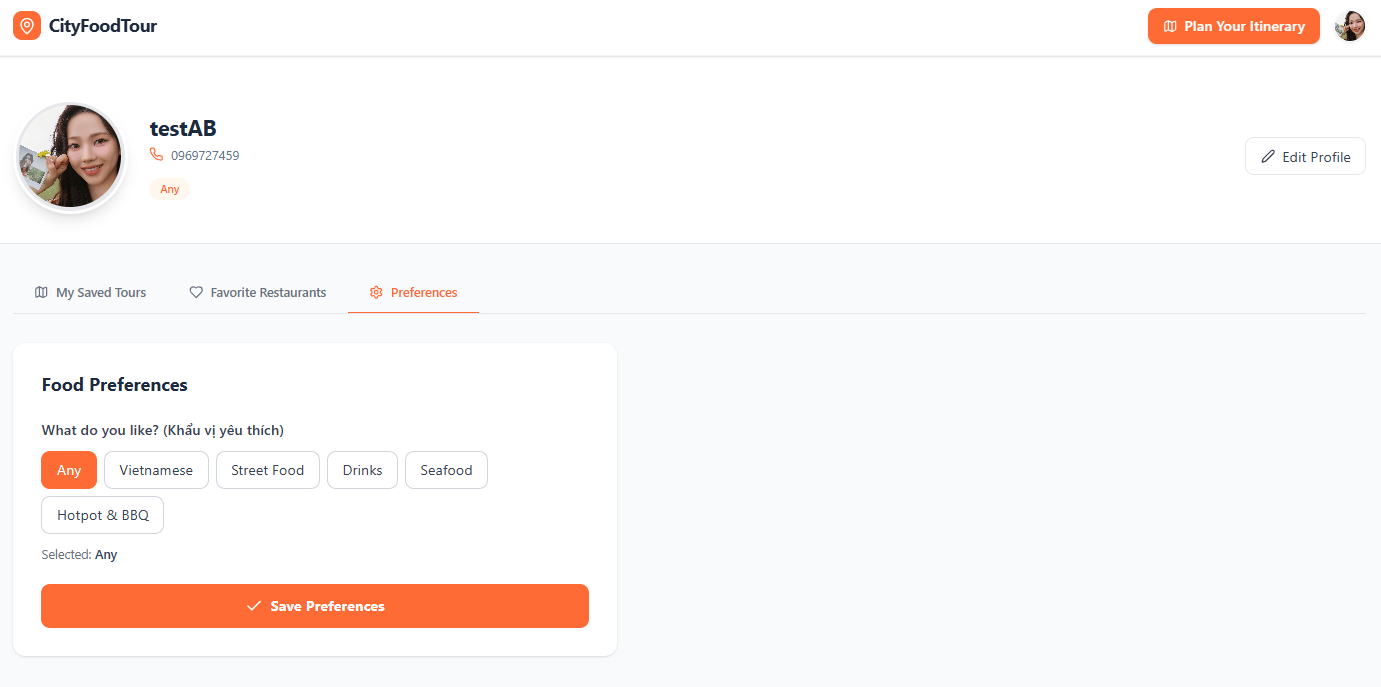
\includegraphics[width=1\textwidth]{img/profile.png}
    \caption{Giao diện hồ sơ người dùng}
\end{figure}

Giao diện hồ sơ người dùng bao gồm các mục chức năng như danh sách food tour đã
lưu, danh sách quán ăn yêu thích và phần thiết lập khẩu vị cá nhân (Preferences). Trong đó, mục thiết lập khẩu vị cho phép người dùng lựa chọn các loại ẩm thực yêu thích nhằm phục vụ cho việc gợi ý quán ăn và food tour phù hợp.

Việc lưu trữ thông tin khẩu vị cá nhân giúp hệ thống cá nhân hóa kết quả đề xuất, tăng mức độ phù hợp của các quán ăn và hành trình ăn uống được gợi ý. Các thao tác cập nhật được thiết kế đơn giản, giúp người dùng dễ dàng thay đổi tùy chọn và lưu lại thông tin.

Nhìn chung, giao diện hồ sơ người dùng được thiết kế gọn gàng, trực quan và nhất
quán với tổng thể hệ thống, đóng vai trò hỗ trợ quan trọng trong việc cá nhân hóa trải nghiệm người dùng và nâng cao hiệu quả của các chức năng đề xuất.

\subsubsubsection{Giao diện hỗ trợ xây dựng FoodTour}
Hình 5.11 minh họa giao diện hỗ trợ xây dựng food tour của hệ thống CityFoodTour.Giao diện này cung cấp các chức năng tìm kiếm quán ăn, food tour và món ăn nhằm hỗ trợ người dùng lựa chọn và xây dựng hành trình ăn uống phù hợp.

Thông qua các mục chức năng được bố trí ở thanh bên, người dùng có thể dễ dàng
chuyển đổi giữa các hình thức tìm kiếm khác nhau trong quá trình lập kế hoạch.
Thiết kế này giúp người dùng từng bước xây dựng food tour mà không bị quá tải
thông tin trên một màn hình duy nhất.

\begin{figure}[H]
    \centering
    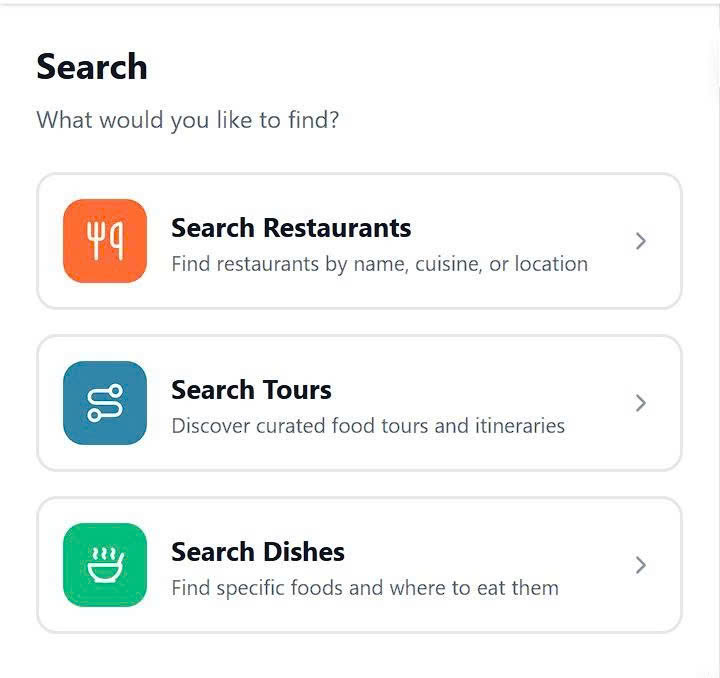
\includegraphics[width=0.8\textwidth]{img/foodtour.png}
    \caption{Giao diện hỗ trợ xây dựng FoodTour}
\end{figure}

\subsubsubsection{Giao diện chi tiết FoodTour}
Giao diện chi tiết food tour được thiết kế nhằm cung cấp đầy đủ thông tin về một
hành trình ăn uống cụ thể, hỗ trợ người dùng hiểu rõ nội dung và cấu trúc của food tour trước khi lựa chọn hoặc sử dụng.

Hình 5.12 minh họa giao diện chi tiết food tour của hệ thống CityFoodTour. Tại khu vực đầu trang, giao diện hiển thị hình ảnh minh họa, tên food tour, điểm đánh giá trung bình, thời lượng dự kiến, số lượng điểm dừng và tổng quãng đường di chuyển. Các thông tin này giúp người dùng nhanh chóng nắm bắt quy mô và đặc điểm tổng quan của hành trình.

\begin{figure}[H]
    \centering
    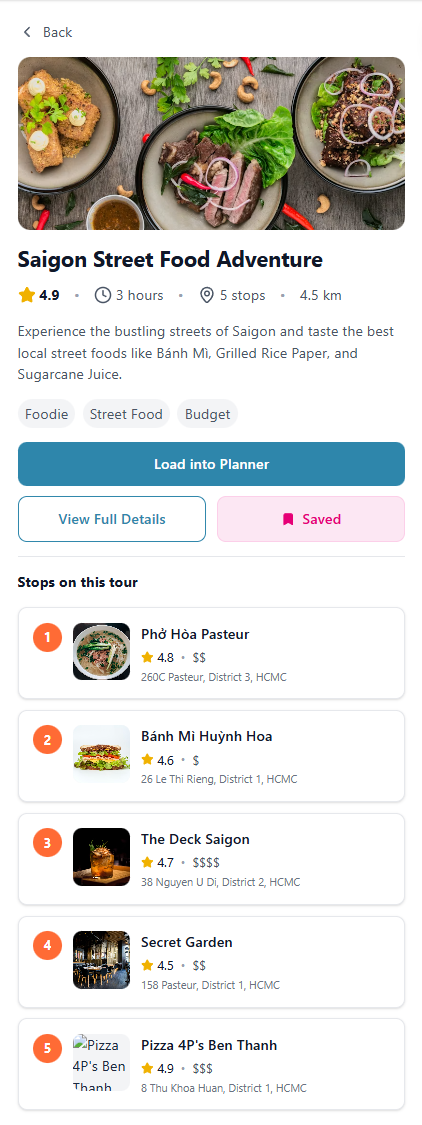
\includegraphics[width=0.5\textwidth]{img/tourdetail.png}
    \caption{Giao diện chi tiết FoodTour}
\end{figure}

Bên dưới phần thông tin tổng quan, giao diện cung cấp mô tả ngắn về nội dung food tour, giúp người dùng hiểu rõ chủ đề và trải nghiệm mà hành trình mang lại. Các thẻ nhãn (tags) được sử dụng để phân loại food tour theo loại hình ẩm thực và phong cách, hỗ trợ việc tìm kiếm và gợi ý.

Giao diện chi tiết food tour cho phép người dùng thực hiện các thao tác như lưu food tour, xem chi tiết đầy đủ hoặc tải food tour vào trình lập kế hoạch nhằm phục vụ việc xây dựng hành trình cá nhân. Các chức năng này giúp tăng khả năng tái sử dụng và chia sẻ food tour trong hệ thống.

Danh sách các điểm dừng trong food tour được hiển thị theo thứ tự ghé thăm, mỗi
điểm dừng bao gồm thông tin cơ bản về quán ăn như tên, địa chỉ, mức giá và điểm
đánh giá. Cách trình bày theo thứ tự giúp người dùng dễ dàng hình dung cấu trúc
hành trình và các địa điểm sẽ ghé thăm.

Nhìn chung, giao diện chi tiết food tour được thiết kế trực quan, đầy đủ thông tin và nhất quán với tổng thể hệ thống, đóng vai trò quan trọng trong việc hỗ trợ người dùng khám phá, lựa chọn và sử dụng các hành trình ăn uống một cách hiệu quả.